% Created by tikzDevice version 0.12.6 on 2024-08-01 12:50:20
% !TEX encoding = UTF-8 Unicode
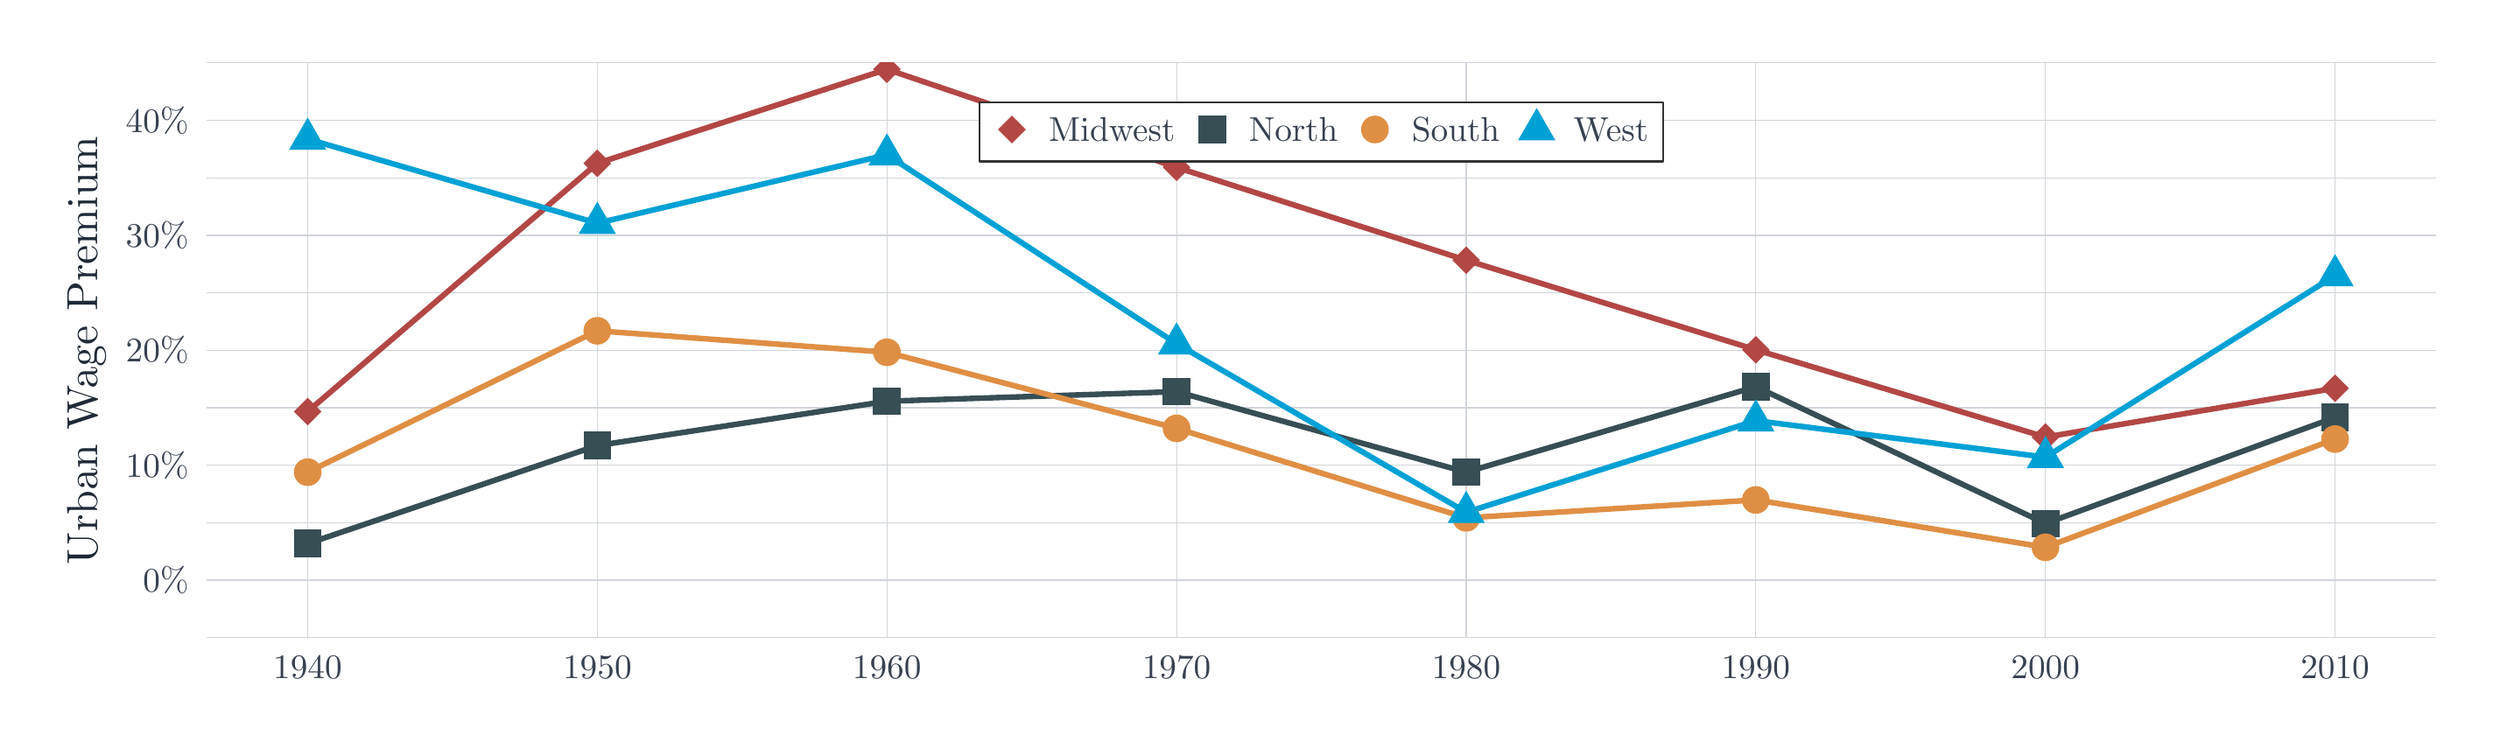
\begin{tikzpicture}[x=1pt,y=1pt]
\definecolor{fillColor}{RGB}{255,255,255}
\path[use as bounding box,fill=fillColor] (0,0) rectangle (1011.78,289.08);
\begin{scope}
\path[clip] (  0.00,  0.00) rectangle (1011.78,289.08);
\definecolor{drawColor}{RGB}{255,255,255}

\path[draw=drawColor,line width= 0.8pt,line join=round,line cap=round,fill=fillColor] (  0.00,  0.00) rectangle (1011.78,289.08);
\end{scope}
\begin{scope}
\path[clip] ( 75.16, 35.76) rectangle (995.78,273.08);
\definecolor{drawColor}{RGB}{255,255,255}
\definecolor{fillColor}{RGB}{255,255,255}

\path[draw=drawColor,line width= 0.8pt,line join=round,line cap=round,fill=fillColor] ( 75.16, 35.76) rectangle (995.78,273.08);
\definecolor{drawColor}{RGB}{209,213,219}

\path[draw=drawColor,line width= 0.4pt,line join=round] ( 75.16, 35.76) --
	(995.78, 35.76);

\path[draw=drawColor,line width= 0.4pt,line join=round] ( 75.16, 83.22) --
	(995.78, 83.22);

\path[draw=drawColor,line width= 0.4pt,line join=round] ( 75.16,130.69) --
	(995.78,130.69);

\path[draw=drawColor,line width= 0.4pt,line join=round] ( 75.16,178.15) --
	(995.78,178.15);

\path[draw=drawColor,line width= 0.4pt,line join=round] ( 75.16,225.62) --
	(995.78,225.62);

\path[draw=drawColor,line width= 0.4pt,line join=round] ( 75.16,273.08) --
	(995.78,273.08);

\path[draw=drawColor,line width= 0.4pt,line join=round] ( 75.16, 59.49) --
	(995.78, 59.49);

\path[draw=drawColor,line width= 0.4pt,line join=round] ( 75.16,106.95) --
	(995.78,106.95);

\path[draw=drawColor,line width= 0.4pt,line join=round] ( 75.16,154.42) --
	(995.78,154.42);

\path[draw=drawColor,line width= 0.4pt,line join=round] ( 75.16,201.88) --
	(995.78,201.88);

\path[draw=drawColor,line width= 0.4pt,line join=round] ( 75.16,249.35) --
	(995.78,249.35);

\path[draw=drawColor,line width= 0.4pt,line join=round] (117.01, 35.76) --
	(117.01,273.08);

\path[draw=drawColor,line width= 0.4pt,line join=round] (236.57, 35.76) --
	(236.57,273.08);

\path[draw=drawColor,line width= 0.4pt,line join=round] (356.13, 35.76) --
	(356.13,273.08);

\path[draw=drawColor,line width= 0.4pt,line join=round] (475.69, 35.76) --
	(475.69,273.08);

\path[draw=drawColor,line width= 0.4pt,line join=round] (595.25, 35.76) --
	(595.25,273.08);

\path[draw=drawColor,line width= 0.4pt,line join=round] (714.81, 35.76) --
	(714.81,273.08);

\path[draw=drawColor,line width= 0.4pt,line join=round] (834.37, 35.76) --
	(834.37,273.08);

\path[draw=drawColor,line width= 0.4pt,line join=round] (953.93, 35.76) --
	(953.93,273.08);
\definecolor{drawColor}{RGB}{178,71,69}

\path[draw=drawColor,line width= 2.3pt,line join=round] (117.01,129.12) --
	(236.57,231.62) --
	(356.13,270.46) --
	(475.69,229.96) --
	(595.25,191.62) --
	(714.81,154.63) --
	(834.37,118.57) --
	(953.93,138.73);
\definecolor{drawColor}{RGB}{55,78,85}

\path[draw=drawColor,line width= 2.3pt,line join=round] (117.01, 74.59) --
	(236.57,115.08) --
	(356.13,133.37) --
	(475.69,137.33) --
	(595.25,104.09) --
	(714.81,139.39) --
	(834.37, 82.88) --
	(953.93,126.71);
\definecolor{drawColor}{RGB}{223,143,68}

\path[draw=drawColor,line width= 2.3pt,line join=round] (117.01,104.09) --
	(236.57,162.47) --
	(356.13,153.60) --
	(475.69,122.17) --
	(595.25, 85.23) --
	(714.81, 92.62) --
	(834.37, 73.06) --
	(953.93,117.76);
\definecolor{drawColor}{RGB}{0,161,213}

\path[draw=drawColor,line width= 2.3pt,line join=round] (117.01,241.66) --
	(236.57,206.91) --
	(356.13,235.15) --
	(475.69,157.14) --
	(595.25, 87.53) --
	(714.81,125.35) --
	(834.37,110.28) --
	(953.93,185.27);
\definecolor{fillColor}{RGB}{178,71,69}

\path[fill=fillColor] (111.30,129.12) --
	(117.01,134.83) --
	(122.72,129.12) --
	(117.01,123.41) --
	cycle;
\definecolor{fillColor}{RGB}{55,78,85}

\path[fill=fillColor] (111.30, 68.88) --
	(122.72, 68.88) --
	(122.72, 80.30) --
	(111.30, 80.30) --
	cycle;
\definecolor{fillColor}{RGB}{223,143,68}

\path[fill=fillColor] (117.01,104.09) circle (  5.71);
\definecolor{fillColor}{RGB}{0,161,213}

\path[fill=fillColor] (117.01,250.54) --
	(124.70,237.22) --
	(109.32,237.22) --
	cycle;
\definecolor{fillColor}{RGB}{178,71,69}

\path[fill=fillColor] (230.86,231.62) --
	(236.57,237.33) --
	(242.28,231.62) --
	(236.57,225.91) --
	cycle;
\definecolor{fillColor}{RGB}{55,78,85}

\path[fill=fillColor] (230.86,109.37) --
	(242.28,109.37) --
	(242.28,120.79) --
	(230.86,120.79) --
	cycle;
\definecolor{fillColor}{RGB}{223,143,68}

\path[fill=fillColor] (236.57,162.47) circle (  5.71);
\definecolor{fillColor}{RGB}{0,161,213}

\path[fill=fillColor] (236.57,215.79) --
	(244.26,202.47) --
	(228.88,202.47) --
	cycle;
\definecolor{fillColor}{RGB}{178,71,69}

\path[fill=fillColor] (350.42,270.46) --
	(356.13,276.17) --
	(361.84,270.46) --
	(356.13,264.75) --
	cycle;
\definecolor{fillColor}{RGB}{55,78,85}

\path[fill=fillColor] (350.42,127.66) --
	(361.84,127.66) --
	(361.84,139.08) --
	(350.42,139.08) --
	cycle;
\definecolor{fillColor}{RGB}{223,143,68}

\path[fill=fillColor] (356.13,153.60) circle (  5.71);
\definecolor{fillColor}{RGB}{0,161,213}

\path[fill=fillColor] (356.13,244.03) --
	(363.82,230.71) --
	(348.44,230.71) --
	cycle;
\definecolor{fillColor}{RGB}{178,71,69}

\path[fill=fillColor] (469.98,229.96) --
	(475.69,235.67) --
	(481.40,229.96) --
	(475.69,224.25) --
	cycle;
\definecolor{fillColor}{RGB}{55,78,85}

\path[fill=fillColor] (469.98,131.62) --
	(481.40,131.62) --
	(481.40,143.04) --
	(469.98,143.04) --
	cycle;
\definecolor{fillColor}{RGB}{223,143,68}

\path[fill=fillColor] (475.69,122.17) circle (  5.71);
\definecolor{fillColor}{RGB}{0,161,213}

\path[fill=fillColor] (475.69,166.02) --
	(483.38,152.70) --
	(468.00,152.70) --
	cycle;
\definecolor{fillColor}{RGB}{178,71,69}

\path[fill=fillColor] (589.54,191.62) --
	(595.25,197.33) --
	(600.96,191.62) --
	(595.25,185.91) --
	cycle;
\definecolor{fillColor}{RGB}{55,78,85}

\path[fill=fillColor] (589.54, 98.38) --
	(600.96, 98.38) --
	(600.96,109.80) --
	(589.54,109.80) --
	cycle;
\definecolor{fillColor}{RGB}{223,143,68}

\path[fill=fillColor] (595.25, 85.23) circle (  5.71);
\definecolor{fillColor}{RGB}{0,161,213}

\path[fill=fillColor] (595.25, 96.41) --
	(602.94, 83.09) --
	(587.56, 83.09) --
	cycle;
\definecolor{fillColor}{RGB}{178,71,69}

\path[fill=fillColor] (709.10,154.63) --
	(714.81,160.34) --
	(720.52,154.63) --
	(714.81,148.92) --
	cycle;
\definecolor{fillColor}{RGB}{55,78,85}

\path[fill=fillColor] (709.10,133.68) --
	(720.52,133.68) --
	(720.52,145.10) --
	(709.10,145.10) --
	cycle;
\definecolor{fillColor}{RGB}{223,143,68}

\path[fill=fillColor] (714.81, 92.62) circle (  5.71);
\definecolor{fillColor}{RGB}{0,161,213}

\path[fill=fillColor] (714.81,134.23) --
	(722.50,120.91) --
	(707.12,120.91) --
	cycle;
\definecolor{fillColor}{RGB}{178,71,69}

\path[fill=fillColor] (828.66,118.57) --
	(834.37,124.28) --
	(840.08,118.57) --
	(834.37,112.86) --
	cycle;
\definecolor{fillColor}{RGB}{55,78,85}

\path[fill=fillColor] (828.66, 77.17) --
	(840.08, 77.17) --
	(840.08, 88.59) --
	(828.66, 88.59) --
	cycle;
\definecolor{fillColor}{RGB}{223,143,68}

\path[fill=fillColor] (834.37, 73.06) circle (  5.71);
\definecolor{fillColor}{RGB}{0,161,213}

\path[fill=fillColor] (834.37,119.16) --
	(842.06,105.84) --
	(826.68,105.84) --
	cycle;
\definecolor{fillColor}{RGB}{178,71,69}

\path[fill=fillColor] (948.22,138.73) --
	(953.93,144.44) --
	(959.64,138.73) --
	(953.93,133.02) --
	cycle;
\definecolor{fillColor}{RGB}{55,78,85}

\path[fill=fillColor] (948.22,121.00) --
	(959.64,121.00) --
	(959.64,132.42) --
	(948.22,132.42) --
	cycle;
\definecolor{fillColor}{RGB}{223,143,68}

\path[fill=fillColor] (953.93,117.76) circle (  5.71);
\definecolor{fillColor}{RGB}{0,161,213}

\path[fill=fillColor] (953.93,194.15) --
	(961.62,180.83) --
	(946.24,180.83) --
	cycle;
\end{scope}
\begin{scope}
\path[clip] (  0.00,  0.00) rectangle (1011.78,289.08);
\definecolor{drawColor}{RGB}{55,65,81}

\node[text=drawColor,anchor=base east,inner sep=0pt, outer sep=0pt, scale=  1.42] at ( 67.96, 54.59) {0\%};

\node[text=drawColor,anchor=base east,inner sep=0pt, outer sep=0pt, scale=  1.42] at ( 67.96,102.06) {10\%};

\node[text=drawColor,anchor=base east,inner sep=0pt, outer sep=0pt, scale=  1.42] at ( 67.96,149.52) {20\%};

\node[text=drawColor,anchor=base east,inner sep=0pt, outer sep=0pt, scale=  1.42] at ( 67.96,196.99) {30\%};

\node[text=drawColor,anchor=base east,inner sep=0pt, outer sep=0pt, scale=  1.42] at ( 67.96,244.45) {40\%};
\end{scope}
\begin{scope}
\path[clip] (  0.00,  0.00) rectangle (1011.78,289.08);
\definecolor{drawColor}{RGB}{55,65,81}

\node[text=drawColor,anchor=base,inner sep=0pt, outer sep=0pt, scale=  1.42] at (117.01, 18.76) {1940};

\node[text=drawColor,anchor=base,inner sep=0pt, outer sep=0pt, scale=  1.42] at (236.57, 18.76) {1950};

\node[text=drawColor,anchor=base,inner sep=0pt, outer sep=0pt, scale=  1.42] at (356.13, 18.76) {1960};

\node[text=drawColor,anchor=base,inner sep=0pt, outer sep=0pt, scale=  1.42] at (475.69, 18.76) {1970};

\node[text=drawColor,anchor=base,inner sep=0pt, outer sep=0pt, scale=  1.42] at (595.25, 18.76) {1980};

\node[text=drawColor,anchor=base,inner sep=0pt, outer sep=0pt, scale=  1.42] at (714.81, 18.76) {1990};

\node[text=drawColor,anchor=base,inner sep=0pt, outer sep=0pt, scale=  1.42] at (834.37, 18.76) {2000};

\node[text=drawColor,anchor=base,inner sep=0pt, outer sep=0pt, scale=  1.42] at (953.93, 18.76) {2010};
\end{scope}
\begin{scope}
\path[clip] (  0.00,  0.00) rectangle (1011.78,289.08);
\definecolor{drawColor}{RGB}{31,41,55}

\node[text=drawColor,rotate= 90.00,anchor=base,inner sep=0pt, outer sep=0pt, scale=  1.80] at ( 30.15,154.42) {Urban Wage Premium};
\end{scope}
\begin{scope}
\path[clip] (  0.00,  0.00) rectangle (1011.78,289.08);
\definecolor{drawColor}{gray}{0.20}
\definecolor{fillColor}{RGB}{255,255,255}

\path[draw=drawColor,line width= 0.8pt,line join=round,line cap=round,fill=fillColor] (394.47,232.37) rectangle (676.47,256.83);
\end{scope}
\begin{scope}
\path[clip] (  0.00,  0.00) rectangle (1011.78,289.08);
\definecolor{drawColor}{RGB}{255,255,255}
\definecolor{fillColor}{RGB}{255,255,255}

\path[draw=drawColor,line width= 0.8pt,line join=round,line cap=round,fill=fillColor] (400.47,238.37) rectangle (414.92,252.83);
\end{scope}
\begin{scope}
\path[clip] (  0.00,  0.00) rectangle (1011.78,289.08);
\definecolor{fillColor}{RGB}{178,71,69}

\path[fill=fillColor] (401.99,245.60) --
	(407.70,251.31) --
	(413.41,245.60) --
	(407.70,239.89) --
	cycle;
\end{scope}
\begin{scope}
\path[clip] (  0.00,  0.00) rectangle (1011.78,289.08);
\definecolor{drawColor}{RGB}{255,255,255}
\definecolor{fillColor}{RGB}{255,255,255}

\path[draw=drawColor,line width= 0.8pt,line join=round,line cap=round,fill=fillColor] (483.13,238.37) rectangle (497.58,252.83);
\end{scope}
\begin{scope}
\path[clip] (  0.00,  0.00) rectangle (1011.78,289.08);
\definecolor{fillColor}{RGB}{55,78,85}

\path[fill=fillColor] (484.65,239.89) --
	(496.07,239.89) --
	(496.07,251.31) --
	(484.65,251.31) --
	cycle;
\end{scope}
\begin{scope}
\path[clip] (  0.00,  0.00) rectangle (1011.78,289.08);
\definecolor{drawColor}{RGB}{255,255,255}
\definecolor{fillColor}{RGB}{255,255,255}

\path[draw=drawColor,line width= 0.8pt,line join=round,line cap=round,fill=fillColor] (550.35,238.37) rectangle (564.80,252.83);
\end{scope}
\begin{scope}
\path[clip] (  0.00,  0.00) rectangle (1011.78,289.08);
\definecolor{fillColor}{RGB}{223,143,68}

\path[fill=fillColor] (557.58,245.60) circle (  5.71);
\end{scope}
\begin{scope}
\path[clip] (  0.00,  0.00) rectangle (1011.78,289.08);
\definecolor{drawColor}{RGB}{255,255,255}
\definecolor{fillColor}{RGB}{255,255,255}

\path[draw=drawColor,line width= 0.8pt,line join=round,line cap=round,fill=fillColor] (617.13,238.37) rectangle (631.59,252.83);
\end{scope}
\begin{scope}
\path[clip] (  0.00,  0.00) rectangle (1011.78,289.08);
\definecolor{fillColor}{RGB}{0,161,213}

\path[fill=fillColor] (624.36,254.48) --
	(632.05,241.16) --
	(616.67,241.16) --
	cycle;
\end{scope}
\begin{scope}
\path[clip] (  0.00,  0.00) rectangle (1011.78,289.08);
\definecolor{drawColor}{RGB}{55,65,81}

\node[text=drawColor,anchor=base west,inner sep=0pt, outer sep=0pt, scale=  1.42] at (422.92,240.70) {Midwest};
\end{scope}
\begin{scope}
\path[clip] (  0.00,  0.00) rectangle (1011.78,289.08);
\definecolor{drawColor}{RGB}{55,65,81}

\node[text=drawColor,anchor=base west,inner sep=0pt, outer sep=0pt, scale=  1.42] at (505.58,240.70) {North};
\end{scope}
\begin{scope}
\path[clip] (  0.00,  0.00) rectangle (1011.78,289.08);
\definecolor{drawColor}{RGB}{55,65,81}

\node[text=drawColor,anchor=base west,inner sep=0pt, outer sep=0pt, scale=  1.42] at (572.80,240.70) {South};
\end{scope}
\begin{scope}
\path[clip] (  0.00,  0.00) rectangle (1011.78,289.08);
\definecolor{drawColor}{RGB}{55,65,81}

\node[text=drawColor,anchor=base west,inner sep=0pt, outer sep=0pt, scale=  1.42] at (639.59,240.70) {West};
\end{scope}
\end{tikzpicture}
